\section{Limitations of Existing Stream Management Techniques}
\subsection{Limitation 1: No Fully Automatic Stream Management}

\subsubsection{Shortcomings of existing techniques}
 ... Shortcomings of existing techniques: no fully automatic solution yet.  App should assign virtual stream...


\subsubsection{LBA-based technique's problems}
Many existing data separation techniques such as~\cite{AutoStream, HotCold} 
estimate the data lifetime based on the update frequency of LBAs.  
For example, \textsf{\small AutoStream}~\cite{AutoStream} assumes that, if
some LBAs are frequently rewritten by applications, those LBAs hold hot data.
This LBA-based lifetime prediction 
approach, however, does not work well with recent data-intensive 
applications where a majority of
new data are written in an append-only manner.  

In order to illustrate a mismatch between an LBA-based predictor and 
append-only workloads, we analyzed the write pattern of 
RocksDB~\cite{RocksDB}, which is a
popular key-value store based on the LSM-tree algorithm~\cite{LSM}.
Fig.~\ref{fig:lba_lifetime}(a) shows how LBAs may be related 
to data lifetimes\footnote{The lifetime of data is defined 
by the logical time which is the number of writes to the device 
between when the data is first written 
and when the data is invalidated by an overwrite or a TRIM command.}
in RocksDB~\cite{RocksDB}.  
As shown in Fig.~\ref{fig:lba_lifetime}(a), 
there exists no strong correlation between the LBAs and lifetimes in RocksDB.  
This scatter plot is in sharp contrast with one for update workloads 
where a few distinct LBA regions have short lifetimes while others 
have very long lifetimes.

\begin{figure}[t]
	\centering
	\hfill
	%\vspace{-9pt}
	%\captionsetup[subfigure]{margin={0cm,1cm}}
	\subfloat[Lifetime patterns over LBAs]{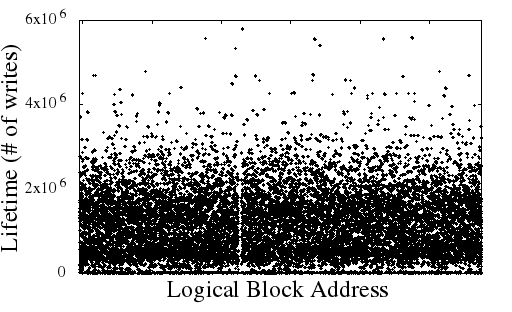
\includegraphics[width=0.215\textwidth]{figure/lba_lifetime2}}  % data from 0/03031641
	\hspace{10pt}
	\subfloat[Lifetime patterns over time]{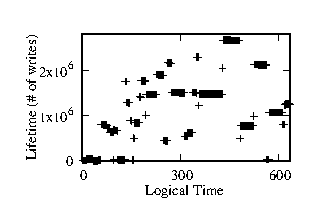
\includegraphics[width=0.21\textwidth]{figure/lifetime_in_chunk}}
	%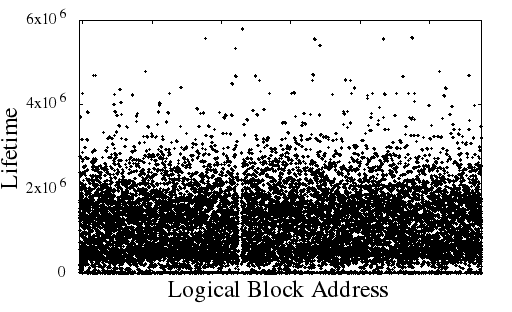
\includegraphics[width=0.9\linewidth]{figure/lba_lifetime} 
	%\vspace{-3pt}
	\caption{Lifetime distributions over addresses and times.} %shane part
	\label{fig:lba_lifetime}
	%\vspace{-20pt}
\end{figure}


We also analyzed 
if the lifetimes of LBAs change under some predictable patterns over time 
although the overall lifetime distribution shows large variances.
Fig.~\ref{fig:lba_lifetime}(b) shows a scatter plot of data lifetimes over the logical time 
for a specific 1-MB chunk with 256 pages. 
As shown in Fig.~\ref{fig:lba_lifetime}(b), 
for the given chuck, data lifetimes vary in a random fashion
(although some temporal locality is observed).
\begin{comment}
Over the logical time, the lifetime of data written to the chunk 
varies in an unpredictable fashion.  
For example, at the logical time 10, the lifetime was 1 but it increases about 
2.6 million around the logical time 450 
followed by a rapid drop around the logical time 600. 
\end{comment}
Our illustration using RocksDB strongly suggests that under append-only
workloads, LBAs are not useful in deciding data lifetimes.


\begin{comment}
In developing PCStream, we started from a simple question: 
how can we extract I/O context from an application? 
For example, in RocksDB, logging, flushing and compaction can be regarded
as different I/O contexts.
RocksDB appends write-ahead logs to storage to ensure data
persistence.  Those logs have short lifetimes because they are quickly deleted
after original data are persistently stored.
The flush module (which materializes the content of a memtable in
DRAM, called an L0 table, to an L1 table in the storage) generates data
with relatively short lifetimes. This is because an L1 table will be flushed to
an L2 table and be removed in the near future. Conversely, a compaction module
writes long-lived data that are unlikely to be removed for a long time.

The above observation implies that, if we are able to know the detailed
behaviors of append-only applications, data with different lifetimes can be
isolated in separate streams in an SSD. As mentioned before, a common
solution~\cite{MultiStream} to realizing this is manually modify an application
code so that each module assigns a unique stream ID to data it generates.
However, owing to considerable implementation efforts required to modify
individual applications, this approach is not widely used in practice.
\end{comment}

\subsection{Limitation 2: Small Number of Available Streams}
It is advantageous to support a large number of streams in order to manage data with different lifetime characteristics as distinct streams.
Therefore, the multi-stream specification defines up to 65536 streams [].
However, the number of streams actually supported by an SSD that implements the specification is limited to 4 to 16[].
This is a limitation that occurs because there are restrictions on the resource required to implement multi-stream. It can be divided into memory, power, and overprovision resource.

First, memory resource may limit the number of multi-stream.
The controller that runs the SSD provides various memories such as TCM, SRAM, and DRAM. 
To optimize the performance, frequently referenced data structures should be located in fast memory.
The size of the data structure associated with a multi-stream is proportional to the number of streams supported and is directly related to performance, so it must be located in fast memory.
However, because of limited memory sizes, such as TCM or SRAM,
 there is a limit to the number of streams that can be supported with good performance.

Second, power resource may limit the number of multi-stream.
SSDs that support multi-stream are used in data centers or storage servers. SSDs use tantalum or electrolytic capacitors as backup power to guarantee data integrity even under sudden power off conditions.
Buffered data that is used to effectively utilize the parallelism of flash ensures reliable write to flash by using backup power during power off detection.
Since the buffered data is managed per stream, its size increases in proportion to the number of streams.
This also limits the number of streams that can be supported because SSDs use limited backup power at the limited PCB size.

Lastly, overprovision resource may limit the number of multi-stream.
As the number of multi-stream support increases, the active point increases. 
For each active point, it is necessary to allocate separate flash blocks.
 As the number of streams increases, it causes a decrease in overprovision area of SSD.
However, since the overprovisioning area of the SSD is limited, if the number of streams becomes too large, there may be a problem of increase of WAF due to overprovision reduction. 
In the case of streams over the number of overprovisioned blocks, flash block allocation  is not possible.
As a result, this makes stream mapping even more difficult.

\subsection{Limitations 3: Heterogeneous Number of Streams Among Different SSDs}
... SSDs have different number of SSDs $->$ Stream managment should be revised whenever SSDs are replaced.
